\section{数据立方}
为有效支持 OLAP 应用,Jim Gray 等人于 1996 年提出一种多维数据计算模型 —— 数据立方 (Data Cube) \cite{gray1997data}。该模型是针对事实表中各维度的所有组合对应的聚集计算,即各个维度不同组合的 GroupBy 计算。它利用各个组合之间的关系,提高计算效率。在 OLAP 术语中,聚合属性称为维属性, 被计算的属性称为度量属性。

如图\ref{fact_table_data_cube} 所示,(a) 为事实表 R, A、B、C 为它的维属性,M 为它的度量属性。(b) 为基于事实表 R 构建的数据立方。(b) 中的每个视图代表某个特定维属性组合的 GroupBy 结果。所有 GroupBy 结果构成数据立方。

\begin{figure}[!htb]
\centering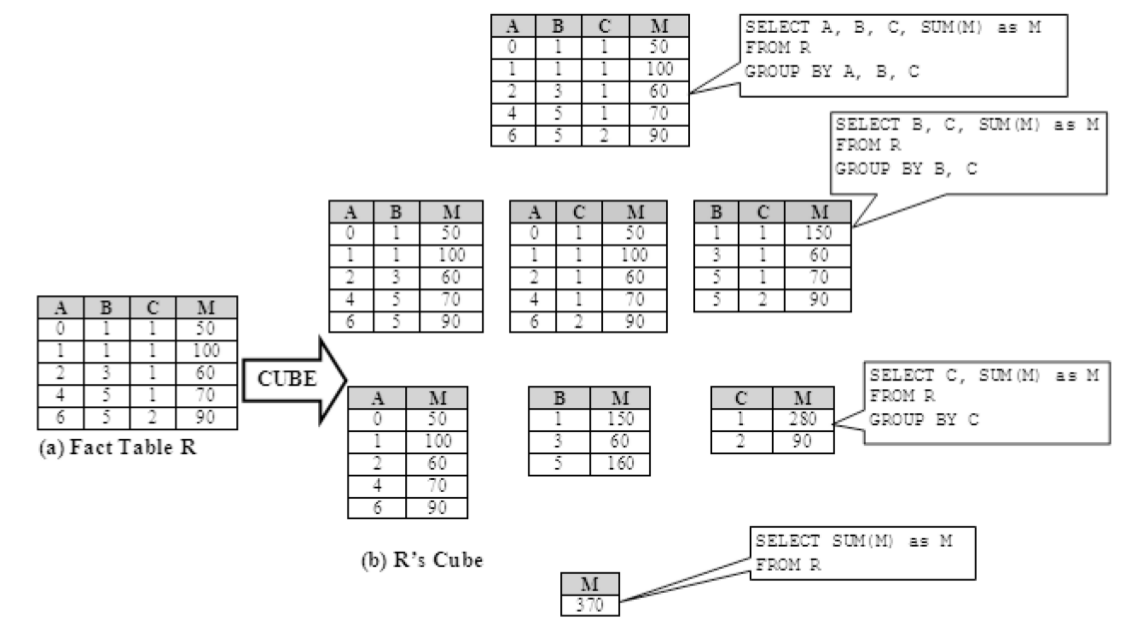
\includegraphics[width=6in]{picture/ch_preliminary/fact_table_data_cube} 
\caption{事实表与数据立方}\label{fact_table_data_cube} 
\end{figure} 

\section{Lattice, Region, Group}

对于图\ref{fact_table_data_cube} 中的所有GroupBy,可用另一种方式表示,如图\ref{abc_lattice} 所示,这种结构称为 Lattice。

\begin{figure}[!htb]
\centering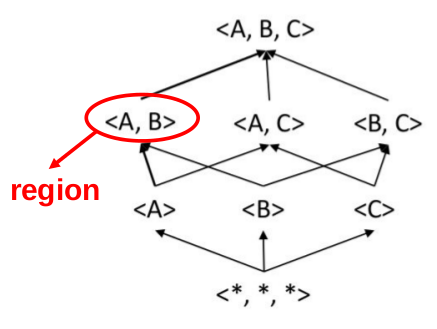
\includegraphics[width=2in]{picture/ch_preliminary/abc_lattice} 
\caption{ABC Lattice}\label{abc_lattice} 
\end{figure} 

在这个lattice中,有维属性组合对应的所有 GroupBy 类型,每个节点表示一种 GroupBy 类型。在lattice中的每个节点称为一个region,也就是一种 GroupBy 类型。箭头连接的两个节点表示它们有父子关系。例如Region(AB)与Region(A)之间有箭头连接,Region(AB)为父,Region(A)为子,表示GroupBy(A)的结果可从GroupBy(AB)的结果计算获得。

一个 region 内有多个 group。group 指的是一个
region中带有具体值的 GroupBy。例如图\ref{fact_table_data_cube} 中的 GroupBy(A),就有表\ref{groupby_a_table}的结果。

\begin{table}[!ht]
\begin{center}
\begin{tabular}{|c|c|}
\hline 
A & M \\ 
\hline 
0 & 50 \\ 
\hline 
1 & 100 \\ 
\hline 
2 & 60 \\ 
\hline 
4 & 70 \\ 
\hline 
6 & 90 \\ 
\hline 
\end{tabular} 
\end{center}
\caption{GroupBy(A)}\label{groupby_a_table}
\end{table}

在表\ref{groupby_a_table}中,Region(A) 中有5个Group,分别是Group(A=0), Group(A=1), Group(A=2), Group(A=4), Group(A=6)。

从lattice中可见,当一个事实表有 D 个维属性时,它对应的数据立方就会有${2}^{D}$个region,也即有 ${2}^{D}$ 种不同类型的 GroupBy。最简单直接(Naive)的数据立方实现方法,是对每个region进行独立计算并把结果存储起来。对于一张事实表,随着他的维属性数量的增加,它相对应的数据立方的计算与存储代价就会呈指数增长。于是,在 OLAP 中,如何从立方计算、立方存储这两个角度高效地实例化数据立方已成为业界内广泛讨论的一个研究课题。


\section{度量}

度量,即对GroupBy的多条数据进行聚合计算,例如SUM,AVG,MEDIAN等。

度量函数一般分为三大类, 分别是分布度量(Distributive),代数度量(Algebraic)和整体性度量(Holistic)。

以下使用一个二维的数据集$\left\{ {X}_{ij}|i=1,...I; j=1,...J \right\}$分别说明这三种度量函数的区别。

\begin{itemize}

\item \textbf{分布度量}

对于分布度量函数 F(),如果存在一个辅助函数 G() 能令 $F(\text\{ {X}_{i,j} \text\}) = G(\text\{ F(\text\{ {X}_{i,j}|i=1,...,I \text\})|j=1,...J \text\})$,则度量函数 F() 为分布度量函数。常见的分布度量函数有 COUNT(), MIN(), MAX(), SUM()。大部分分布度量函数中 $F=G$,但COUNT() 除外。在COUNT()度量函数中,$G=SUM()$。

\item \textbf{代数度量}

对于代数度量函数 F(),如果存在辅助两个函数 G() 和 H(),其中 G() 的输出结果是固定数量的 M 条记录,并且满足$F(\text\{ {X}_{i,j} \text\}) = H(\text\{ G(\text\{ {X}_{i,j}|i=1,...,I \text\})|j=1,...J \text\})$。常见的代数度量函数有AVG(),MaxN(),MinN(),标准差等。例如对于AVG(),函数G()的输出是子集的和以及数量,H()函数则把将各个子集的和相加再除以数量的总和。代数度量的关键是,函数G()的输出结果的数据量是固定的。例如AVG(),无论数据怎么划分,函数G()的输出都是两个值,一个是和,另一个是数量。

\item \textbf{整体性度量}

对于整体性性度量函数 F(),其中间结果,即各个子集的计算结果的数据量大小是不确定的。常见的整体性度量有Median(), Mode(), RANK(), DISTINCT()等。例如使用 DISTINCT()计算一个数列中出现多少不同的数值。若将该数列随意划分,那么每个子数列输出的中间结果仍可能是一个列表,该列表记录了子数列出现哪些数值,即将重复的数值去除。然后再对这些中间结果计算 DISTINCT()。在最坏的情况下,每个子数列输出的中间结果可能就是它本身,因为无重复的数值。

\end{itemize}

之所以要对度量函数进行分类是因为其会影响数据的划分以及数据立方的计算。论文研究的环境是分布式,因此数据划分是必然的。对于以上三种度量,在分布度量与代数度量下,数据无论如何划分,使用辅助函数都能计算出最终结果,并且中间结果的数据量是确定的。但对于整体性度量,数据无法随意划分,或者数据的随意划分对其计算的意义并不大,因为中间结果数据量的不确定导致中间数据的维护代价可能很大。然而这并不代表数据不能划分。在后面的章节中会提到,对于整体性度量按照一定的方法对数据进行划分,也能令中间结果的数据大小是确定的。为了方便,在之后的阐述中,将分布度量与代数度量都归为代数度量。